\subsection{Motivation}
\label{sec:zeta_motivation}

The simulated momenta $P_L=-1,\ldots,-4$ correspond to the finite Collins-Soper parameters $\hat\zeta=0.090772$, $0.294367$, $0.539684$ and $0.785756$. A quantitative comparison with phenomenological and experimental TMD studies that employ QCD factorization requires much larger Collins-Soper parameters, $\hat\zeta\gg1$. The limit $\hat\zeta\to\infty$ corresponds to a light-like staple direction $v$. For the Sivers shift, where the soft factors in the TMD definitions~\cite{Ji:2004wu,Aybat:2011zv,CollinsBook2011} cancel, large values of $\hat\zeta$ are accessed through large nucleon momenta. This limit is not accessible on the lattice in practice, so we extrapolate results for a limited range of $\hat\zeta$. From the perturbative prediction for the $\zeta$ dependence~\cite{Aybat:2011zv} we expect the ratios of TMDs to become independent of $\hat\zeta$ as $\hat\zeta\to\infty$. At fixed $|\vect b_T|=3a\approx0.34$~fm, we evaluate the reconstructed amplitudes, the TMD combinations $\tilde f_1^{(0)}=2\tAmp_{2B}^{[x]}$ and $\tilde f_{1T}^{\perp(1)}=-2\tAmp_{12B}^{[x]\text{Re}}$, and the Sivers shift as functions of $x$ at each simulated momentum. Plotted against $1/\hat\zeta$, all of them vary systematically with the momentum (Figs.~\ref{fig:zetahat_slices_amps} and~\ref{fig:zetahat_slices}).

\begin{figure*}[!t]
\centering
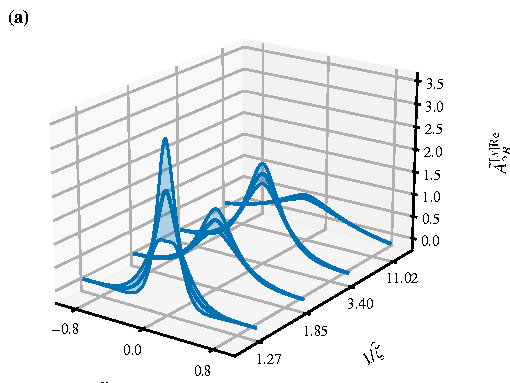
\includegraphics[width=\panelw]{figures/panels/zeta/zeta_ReA2B.pdf}\hfill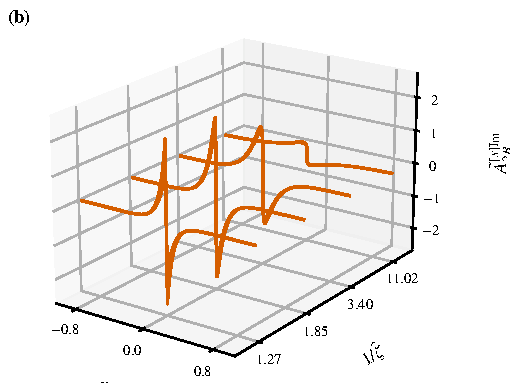
\includegraphics[width=\panelw]{figures/panels/zeta/zeta_ImA2B.pdf}\par
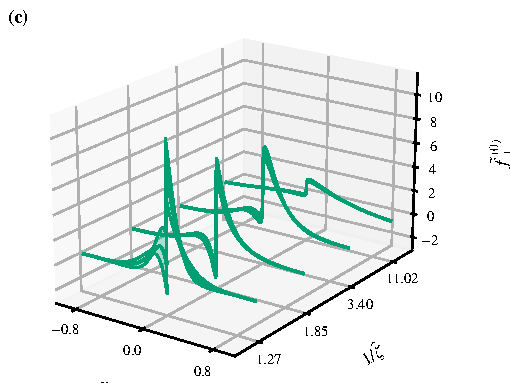
\includegraphics[width=\panelw]{figures/panels/zeta/zeta_f1.pdf}\hfill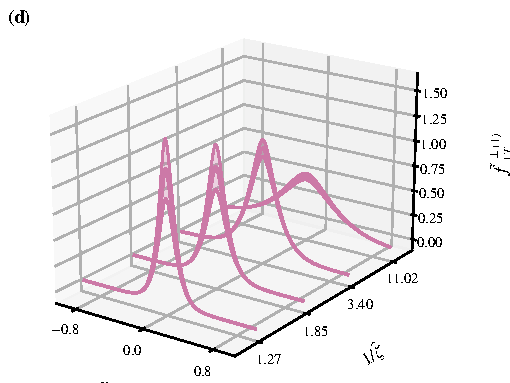
\includegraphics[width=\panelw]{figures/panels/zeta/zeta_f1T.pdf}
\caption{Reconstructed amplitudes (a) $\tAmp_{2B}^{[x]\text{Re}}$ and (b) $\tAmp_{2B}^{[x]\text{Im}}$, and the TMD combinations (c) $\tilde f_1^{(0)}=2\tAmp_{2B}^{[x]}$ and (d) $\tilde f_{1T}^{\perp(1)}=-2\tAmp_{12B}^{[x]\text{Re}}$ at $|\vect b_T|=3a\approx0.34$~fm for the four simulated momenta, against $x$ and $1/\hat\zeta$. The four slices are drawn at equal spacing and labeled by their $1/\hat\zeta$. Bands are Jackknife errors.}
\label{fig:zetahat_slices_amps}
\end{figure*}

\begin{figure*}[!t]
\centering
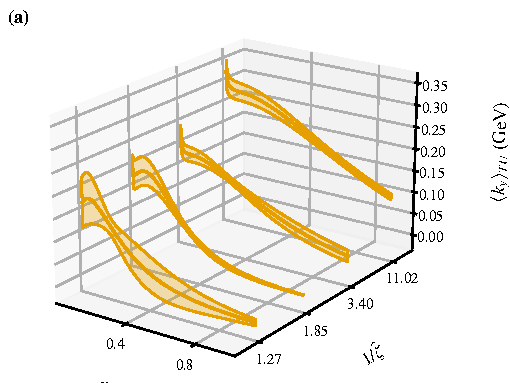
\includegraphics[width=\panelw]{figures/panels/zeta/zeta_ky.pdf}\hfill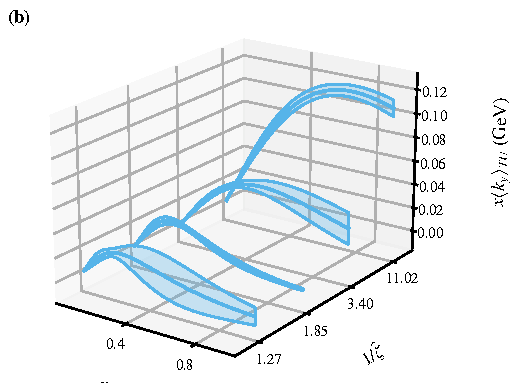
\includegraphics[width=\panelw]{figures/panels/zeta/zeta_xky.pdf}
\caption{Sivers shift (a) $\langle k_y\rangle_{TU}$ and (b) $x\langle k_y\rangle_{TU}$ at $|\vect b_T|=3a\approx0.34$~fm for the four simulated momenta, against $x$ and $1/\hat\zeta$ ($x\ge0$). The four slices are drawn at equal spacing and labeled by their $1/\hat\zeta$.}
\label{fig:zetahat_slices}
\end{figure*}

\subsection{Extrapolation of the fit parameters}
\label{sec:zeta_extrapolation}

The lowest simulated momentum, $P_L=-1$, lies at $1/\hat\zeta=11.02$, far from the other three ($1/\hat\zeta=3.40$, $1.85$, $1.27$) and from the asymptotic region $1/\hat\zeta\to0$ that the extrapolation targets. A single point that far out would dominate the two-parameter fits introduced below and bias the extrapolated intercept rather than constrain it. We therefore exclude $P_L=-1$ and extrapolate using only the three higher momenta. Rather than extrapolate the amplitudes point by point in $x$, we extrapolate the fit parameters of the global simultaneous-fit models directly. In these models $c$ multiplies $b_L^2=(P\cdot b)^2/P_L^2$ and the coefficient of the odd amplitude $\tAmp_{2B}^{\text{Im}}$ multiplies $b_L=(P\cdot b)/(-P_L)$, so the parameters $c$ of the three amplitudes are first rescaled by $1/P_L^2$ and the coefficient of $\tAmp_{2B}^{\text{Im}}$ by $1/P_L$. After rescaling, they multiply powers of the invariant $P\cdot b$ directly, so all three momenta can be fit on a common footing. For the $\hat\zeta$ dependence of each rescaled parameter we tested two functional forms, as explored in Ref.~\cite{Musch:2011er},
\begin{equation}
p(\hat\zeta)=p_0+\frac{p_1}{\hat\zeta}\quad\text{and}\quad p(\hat\zeta)=p_0+\frac{p_1}{\hat\zeta^{2}}
\label{eq:zeta_ansatz}
\end{equation}
using correlated Jackknife fits to the three momenta. The two forms give $\chi^2/\text{dof}$ of the same order, with a mean over the twelve parameters of $1.36$ for $1/\hat\zeta$ and $2.04$ for $1/\hat\zeta^2$, and the quadratic form is lower for six of them. The largest difference is for the coefficient of $b_L$ in $\tAmp_{2B}^{\text{Im}}$, with $3.1$ against $12.1$, and its intercept is $-0.0586(35)$ for $1/\hat\zeta^2$ and $-0.0023$ for $1/\hat\zeta$, so the choice of form changes this intercept by far more than its Jackknife error. We use the quadratic form for all parameters (Appendix~\ref{app:param_extrap}, Figs.~\ref{fig:param_extrap} and~\ref{fig:param_extrap_j}). The extrapolated value of each parameter is its fitted intercept $p_0$. With only three momenta and two parameters per fit, this extrapolation has one degree of freedom, and its systematic uncertainty is not captured by the Jackknife errors.
% TODO(Hari): state why the quadratic form is adopted; the lower-chi2 argument does not hold (python_fits/logs/zeta_ansatz_compare.log)

\subsection{Extrapolated amplitudes and Sivers shift}
\label{sec:extrapolated_sivers}

Reconstructing the amplitudes from the extrapolated parameters gives $\tilde f_1^{(0)}$, $\tilde f_{1T}^{\perp(1)}$ and the Sivers shift at $\hat\zeta\to\infty$ (Figs.~\ref{fig:extrap_amps} and~\ref{fig:extrap_sivers}). At $|\vect b_T|=0.34$~fm, $\langle k_y\rangle_{TU}$ peaks at about $0.21$~GeV at small $x$ and falls to near zero by $x\approx0.5$, while $x\langle k_y\rangle_{TU}$ peaks at about $0.02$~GeV near $x\approx0.15$. The overall sign reverses between the SIDIS and DY limits and the magnitude is unchanged. The extrapolated curve differs from all three finite-momentum curves that enter it, including the one at $P_L=-4$. Fig.~\ref{fig:extrap_sivers_3D} shows the dependence on $|\vect b_T|$ between $3a\approx0.34$~fm and $\sqrt{68}\,a\approx0.94$~fm.

Table~\ref{tab:integrals} lists the $x$-integrals of the extrapolated amplitudes at $|\vect b_T|=3a$. Restricting the integration to $x\in[-1,0]$ or $[0,1]$ isolates the antiquark and quark contributions. Because $\tAmp^{[x]\text{Im}}_{2B}$ is odd in $x$ while $\tAmp^{[x]\text{Re}}_{2B}$ and $\tAmp^{[x]\text{Re}}_{12B}$ are even, the two ranges give equal integrals of the real amplitudes and opposite-sign integrals of the imaginary term, so the combined $[-1,1]$ integral of the imaginary term is consistent with zero. The integrals over $[-\infty,\infty]$ and $[-1,1]$ agree within errors, so the extrapolated amplitudes decay fast enough in $x$ that truncating at $|x|=1$ is negligible. The first four rows are unrenormalized, and the multiplicative renormalization cancels only in the ratio in the last row.

\begin{table*}
\caption{$x$-integrals of the extrapolated ($\hat\zeta\to\infty$) amplitudes at $|\vect b_T|=3a\approx0.34$~fm for four integration ranges. The first four rows are unrenormalized.}
\label{tab:integrals}
\begin{ruledtabular}
\begin{tabular}{lcccc}
Integral & $[-\infty,\infty]$ & $[-1,1]$ & $[-1,0]$ & $[0,1]$ \\
\hline
$\int\!dx\,\tAmp^{[x]\text{Re}}_{2B}$ & $0.751(79)$ & $0.751(80)$ & $0.375(40)$ & $0.375(40)$ \\
$\int\!dx\,\tAmp^{[x]\text{Im}}_{2B}$ & $6(96)\!\times\!10^{-17}$ & $3(24)\!\times\!10^{-16}$ & $0.165(27)$ & $-0.169(29)$ \\
$\int\!dx\,\tilde f_1^{(0)}$ & $1.50(16)$ & $1.50(16)$ & $0.421(81)$ & $1.09(11)$ \\
$\int\!dx\,\tilde f_{1T}^{\perp(1)}$ & $0.302(53)$ & $0.302(53)$ & $0.151(27)$ & $0.151(27)$ \\
$\langle k_y\rangle_{TU}$ (GeV) & $0.217(38)$ & $0.217(38)$ & $0.387(89)$ & $0.150(26)$ \\
\end{tabular}
\end{ruledtabular}
\end{table*}

\begin{figure*}[!t]
\centering
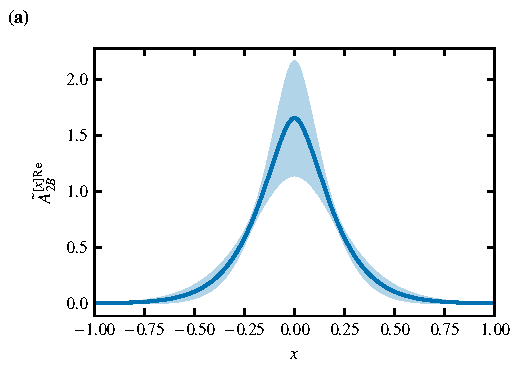
\includegraphics[width=\panelw]{figures/panels/extrap/ext_ReA2B.pdf}\hfill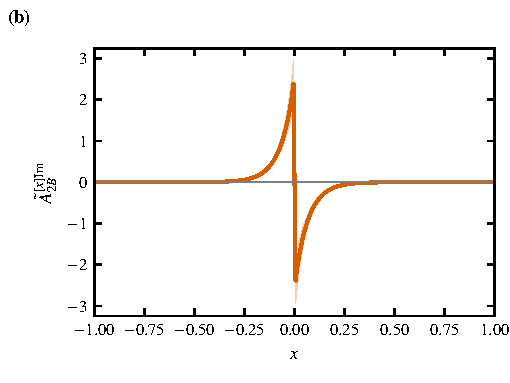
\includegraphics[width=\panelw]{figures/panels/extrap/ext_ImA2B.pdf}\par
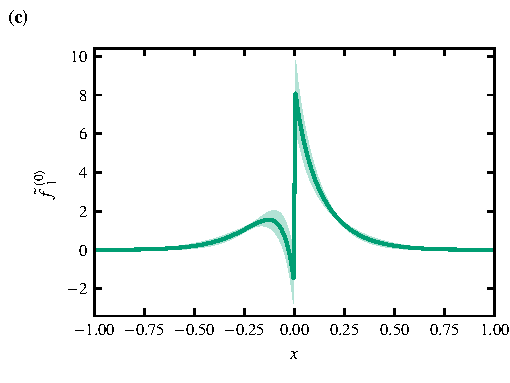
\includegraphics[width=\panelw]{figures/panels/extrap/ext_f1.pdf}\hfill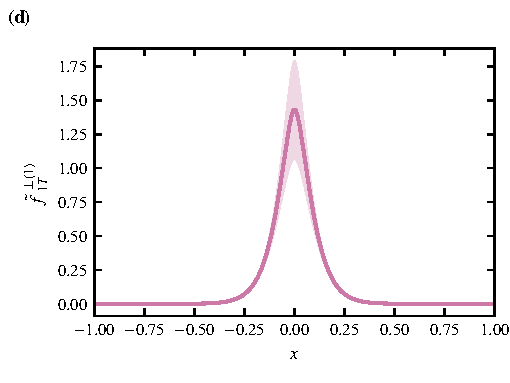
\includegraphics[width=\panelw]{figures/panels/extrap/ext_f1T.pdf}
\caption{Amplitudes (a) $\tAmp^{[x]\text{Re}}_{2B}$ and (b) $\tAmp^{[x]\text{Im}}_{2B}$ and TMD combinations (c) $\tilde f_1^{(0)}$ and (d) $\tilde f_{1T}^{\perp(1)}$ at $\hat\zeta\to\infty$ for $|\vect b_T|=3a\approx0.34$~fm. Bands are Jackknife uncertainties propagated from the extrapolated parameters.}
\label{fig:extrap_amps}
\end{figure*}

\begin{figure*}[!t]
\centering
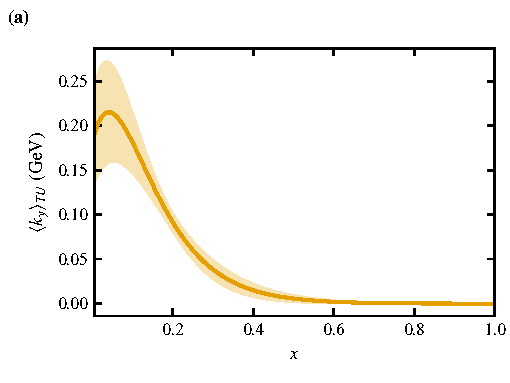
\includegraphics[width=\panelw]{figures/panels/extrap/ext_ky.pdf}\hfill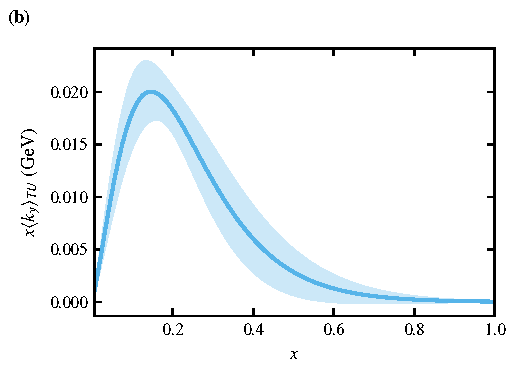
\includegraphics[width=\panelw]{figures/panels/extrap/ext_xky.pdf}
\caption{Sivers shift (a) $\langle k_y\rangle_{TU}$ and (b) $x\langle k_y\rangle_{TU}$ at $\hat\zeta\to\infty$ for $|\vect b_T|=3a\approx0.34$~fm. Bands are Jackknife uncertainties propagated from the extrapolated parameters.}
\label{fig:extrap_sivers}
\end{figure*}

\begin{figure*}[!t]
\centering
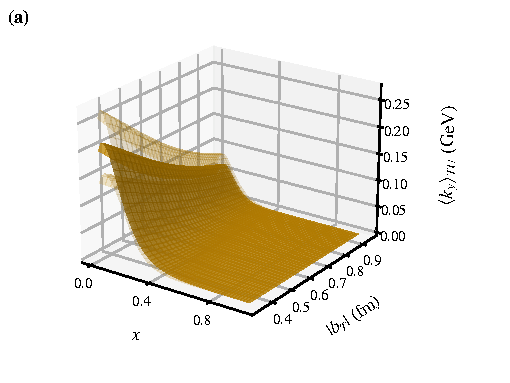
\includegraphics[width=\panelw]{figures/panels/extrap/ext3d_ky.pdf}\hfill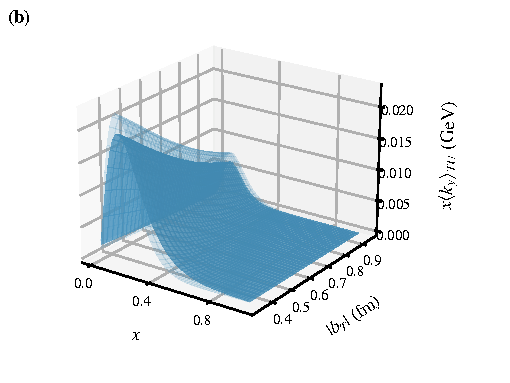
\includegraphics[width=\panelw]{figures/panels/extrap/ext3d_xky.pdf}
\caption{Extrapolated Sivers shift (a) $\langle k_y\rangle_{TU}$ and (b) $x\langle k_y\rangle_{TU}$ as functions of $x\ge0$ and $|\vect b_T|$ from $0.34$ to $0.94$~fm at $\hat\zeta\to\infty$.}
\label{fig:extrap_sivers_3D}
\end{figure*}

\subsection{Factorization in $x$ and $|\vect b_T|$}
\label{sec:factorization}

The global fit couples $(P\cdot b)$ and $b^2$, and the selected models are not products of separate functions of the two variables. We test whether a factorized description, as used in phenomenology, approximates the result. A recent symbolic-regression extraction of the unpolarized TMD from Drell-Yan data finds an $x$-$b_T$ correlation rather than strict separability~\cite{Granger:2026symb}.

We test factorization at two levels. First, we check directly on the lattice data whether an amplitude can be written as a product of longitudinal and transverse profiles, $\tAmp(P\cdot b,b^2)=F(P\cdot b)G(b^2)$. We form $T=\tAmp(P\cdot b,b^2)/\tAmp(P\cdot b=4,b^2)$ and $B=\tAmp(P\cdot b,b^2)/\tAmp(P\cdot b,b^2=18)$, computed on each Jackknife sample. Under factorization $T$ is flat in $b^2$ and $B$ is flat in $P\cdot b$. The limitation of this test is the sampling: at fixed $\eta$ and $P_L$ the lattice points map onto an irregular set of $(P\cdot b,b^2)$ pairs. After the cut $b^2\ge9$, at $\eta|v|/a=8$ and $P_L=-1$ only three values of $P\cdot b$ ($0$, $3$ and $4$) have more than one $b^2$, and no two of these rows share two $b^2$ values. We therefore interpolate in $b^2$ onto a common grid $b^2=18,20,25,32$ (quadratic or linear, with no extrapolation) and find that $T$ is flat near $P\cdot b=0$ but increases monotonically for $P\cdot b=3$, and that $B$ is not flat (Appendix~\ref{app:fact_data}, Fig.~\ref{fig:fact_data}). Because of the sparse sampling and the interpolation this is only a qualitative test, which suggests that factorization is not perfect. At $P_L=-2$ the same points have $P\cdot b=0$, $6$ and $8$, and the reference row of $T$ is $P\cdot b=8$ (Fig.~\ref{fig:fact_data_P2}). The errors are about twice as large as at $P_L=-1$. $T$ for $P\cdot b=6$ rises from $0.81(6)$ at $b^2=18$ to $1.14(8)$ at $b^2=25$ and $2.0(4)$ at $b^2=32$, against $0.92(3)$, $1.17(3)$ and $1.55(9)$ for $P\cdot b=3$ at $P_L=-1$, while $T$ for $P\cdot b=0$ is compatible with $1$ up to $b^2=25$ ($1.01(17)$ at $P_L=-2$). $B$ of $\tAmp_{2B}^{\text{Re}}$ at $b^2=32$ is $0.42(5)$, $0.54(3)$ and $0.22(5)$ at $P\cdot b=0$, $6$ and $8$, against $0.40(3)$, $0.60(1)$ and $0.35(2)$ at $P_L=-1$, so it is not flat at either momentum.

We then ask whether the extrapolated distributions factorize in $x$ and $|\vect b_T|$. For the extrapolated shift $\langle k_y\rangle_{TU}(x,|\vect b_T|)$ we find the pair $g(x)h(|\vect b_T|)$ that minimizes $J=\int dx\,d|\vect b_T|\,(f-gh)^2$ by iterating the self-consistent equation that follows from the stationarity conditions in $g$ and $h$ (Appendix~\ref{app:factorization_metric}), and report the relative distance $\sqrt{J/N}$, with $N=\int dx\,d|\vect b_T|\,f^2$. This is zero for exact factorization. We apply the iteration to each Jackknife sample on a discrete grid of $60$ points in $|\vect b_T|\in[0.3421,0.9403]$~fm and for four $x$-windows. Figs.~\ref{fig:fact_gh} and~\ref{fig:fact_gh_recon} show the optimal factors $g(x)$ and $h(|\vect b_T|)$ and the reconstruction $g\,h$ against the data, and Table~\ref{tab:fact_sivers} shows relative distances of $5.7$--$7.6\%$, nonzero well outside the Jackknife errors and not decreasing as the window moves away from $x=0$. The Sivers shift is therefore close to, but not exactly, factorized.

Factorization in the fit ansatz would require the order $j_X$ and width $d_X$ of the Bessel-type Fourier transform to coincide for the three amplitudes. The extrapolated values are $j_{\text{re}}=2.0667(69)$, $j_{\text{im}}=0.9921(92)$, $j_{\text{reA12B}}=2.0026(40)$ and $d_{\text{re}}=0.139(12)$, $d_{\text{im}}=0.183(14)$, $d_{\text{reA12B}}=0.105(18)$. The $j$ of the imaginary amplitude differs from the other two, and the $d_X$ differ from each other by $1.6\sigma$ to $3.4\sigma$ (errors added in quadrature).

Ratios at fixed $|\vect b_T|$ or fixed $x$ show the same effect directly (Figs.~\ref{fig:fact_ratio_x} and~\ref{fig:fact_ratio_bT}): under exact factorization $R_b(x)=\langle k_y\rangle_{TU}(x,|\vect b_T|)/\langle k_y\rangle_{TU}(x,|\vect b_T|_{\rm ref})$ is flat in $x$ and $R_x(|\vect b_T|)=\langle k_y\rangle_{TU}(x,|\vect b_T|)/\langle k_y\rangle_{TU}(x_{\rm ref},|\vect b_T|)$ is flat in $|\vect b_T|$, and neither is. The same non-flat pattern is present at each finite momentum, so it is a feature of the fitted amplitudes and not of the $\hat\zeta\to\infty$ extrapolation.

The same distance test applied to the individual extrapolated amplitudes for $x\in[0,1]$ gives relative distances of $8$--$19\%$, larger than the $5.7\%$ for the Sivers shift in the same window. For the individual amplitudes the distances decrease as the $x$-window narrows away from $x=0$ (Appendix~\ref{app:factorization_metric}).

We conclude that the extracted Sivers shift is approximately factorized, $F(x)G(|\vect b_T|)$, but not exactly, to about $5.7$--$7.6\%$ in the relative $L_2$ sense. This agrees qualitatively with Ref.~\cite{Granger:2026symb}, where an $x$-$b_T$ cross term survives a sparsity prior. The two results cannot be compared directly: that extraction constrains the TMD for $b_T\lesssim2.5$~GeV$^{-1}$ ($\approx0.49$~fm), our range $0.34$--$0.94$~fm extends well beyond it, and our individual amplitudes are unrenormalized so that only the Sivers-shift ratio is a physical quantity.

\begin{table}
\caption{Relative distance of the extrapolated Sivers shift from its best factorized form $F(x)G(|\vect b_T|)$ for $|\vect b_T|\in[0.3421,0.9403]$~fm.}
\label{tab:fact_sivers}
\begin{ruledtabular}
\begin{tabular}{cc}
$x$-window & Relative distance \\
\hline
$[0.0,1.0]$ & $0.0568(78)$ \\
$[0.1,0.9]$ & $0.0714(95)$ \\
$[0.2,0.8]$ & $0.0758(75)$ \\
$[0.3,0.8]$ & $0.0620(88)$ \\
\end{tabular}
\end{ruledtabular}
\end{table}

\begin{figure*}[!t]
\centering
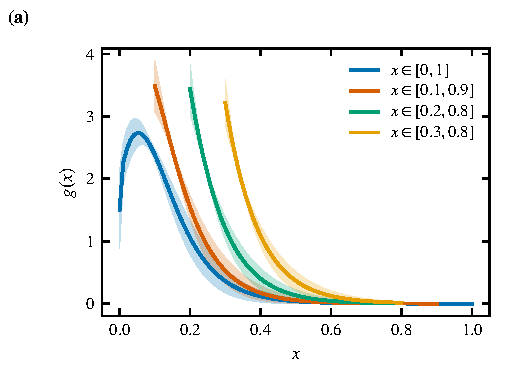
\includegraphics[width=\panelw]{figures/panels/fact/gh_g.pdf}\hfill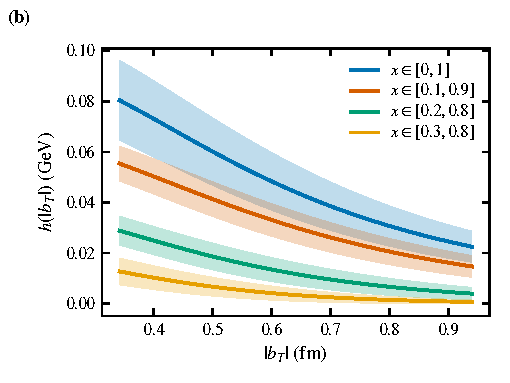
\includegraphics[width=\panelw]{figures/panels/fact/gh_h.pdf}
\caption{Optimal separable factors (a) $g(x)$ and (b) $h(|\vect b_T|)$ for the four $x$-windows of Table~\ref{tab:fact_sivers}.}
\label{fig:fact_gh}
\end{figure*}

\begin{figure}[!t]
\centering
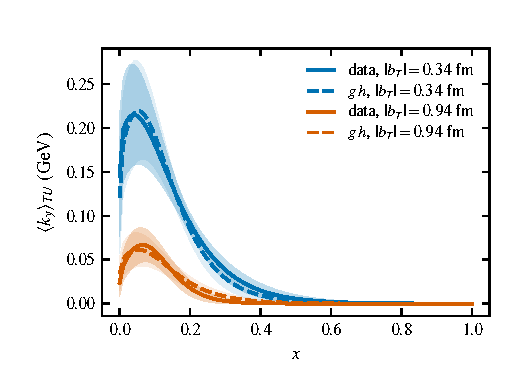
\includegraphics[width=\panelw]{figures/panels/fact/gh_recon.pdf}
\caption{Reconstruction $g\,h$ (dashed) against the extrapolated Sivers shift (solid) at the smallest and largest $|\vect b_T|$, for the window $x\in[0,1]$.}
\label{fig:fact_gh_recon}
\end{figure}

\begin{figure}
\centering
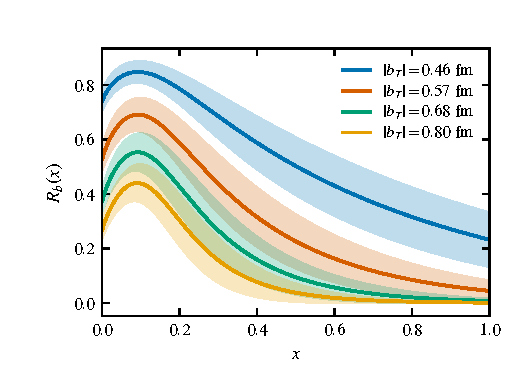
\includegraphics[width=\panelw]{figures/panels/fact/ratio_x.pdf}
\caption{$R_b(x)$ with $|\vect b_T|_{\rm ref}=0.34$~fm for four values of $|\vect b_T|$. Each curve rises from its $x\to0$ value to a peak near $x\approx0.1$ and then decays instead of staying flat.}
\label{fig:fact_ratio_x}
\end{figure}

\begin{figure}
\centering
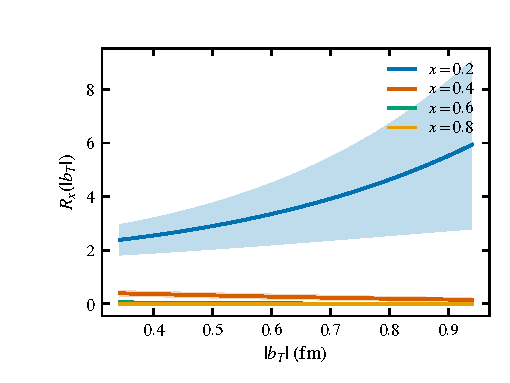
\includegraphics[width=\panelw]{figures/panels/fact/ratio_bT.pdf}
\caption{$R_x(|\vect b_T|)$ with $x_{\rm ref}=0.3$ for four values of $x$. The $x=0.2$ curve changes by more than a factor of two across the fitted range.}
\label{fig:fact_ratio_bT}
\end{figure}
